% --------------------------------------------------------------
% This is all preamble stuff that you don't have to worry about.
% Head down to where it says "Start here"
% --------------------------------------------------------------
% Please add the following required packages to your document preamble:

\documentclass[12pt]{article}

\usepackage[margin=1in]{geometry}
\usepackage{amsmath,amsthm,amssymb}
\usepackage{graphicx}
\usepackage{subcaption}
\usepackage{algorithmicx}
\usepackage{algorithm}
\usepackage{algpseudocode}
\usepackage[colorlinks,linkcolor=blue]{hyperref}
\usepackage[noabbrev]{cleveref}
\usepackage{courier}
\usepackage{listings}
\usepackage{booktabs}


\oddsidemargin 0in
\evensidemargin 0in
\textwidth 6.5in
\topmargin -0.3in
\textheight 9.0in

\newcommand{\ignore}[1]{}
\def\pp{\par\noindent}

\newcommand{\assignment}[4]{
\thispagestyle{plain}
\newpage
\setcounter{page}{1}
\noindent
\begin{center}
\framebox{ \vbox{ \hbox to 6.28in
{CIS 419/519: Applied Machine Learning \hfill #1}
\vspace{4mm}
\hbox to 6.28in
{\hspace{2.5in}\large\bf\mbox{Homework #2}}
\vspace{4mm}
\hbox to 6.28in
{{\it Handed Out: #3 \hfill Due: #4}}
}}
\end{center}
}

\makeatletter
\renewcommand{\fnum@algorithm}{\fname@algorithm}
\makeatother

\lstset{basicstyle=\footnotesize\ttfamily,breaklines=true}
\lstset{framextopmargin=50pt,frame=bottomline}


\begin{document}
\assignment{Spring 2023}{5}{April 5}{April 19, 7:59 p.m.}

% --------------------------------------------------------------
%                         Start here
% --------------------------------------------------------------

\begin{itemize}
\item {\bf Your Name:}  \textit{Qihang Dai}
\item {\bf Your PennKey:} \textit{ahgdyycc}
\item {\bf Your PennID:} \textit{78803164}
\end{itemize}

\section{Multiple Choice \& Written Questions}

\begin{enumerate}
\item
\begin{enumerate}
\item bob loves cookie
\item 
$lnP(w1 = loves, w2 = cookie | w0 = bob)$ = $lnP(w1 = loves | w0 = bob)$ +  $lnP(w2 = cookie | w1 = loves, w0 = bob)$
= $ln0.5$ + $ln0.4$ = $ln0.2$ = 

$lnP(w1 = hates, w2 = cookie | w0 = bob)$ = $lnP(w1 = hates | w0 = bob)$ +  $lnP(w2 = cookie | w1 = hates, w0 = bob)$
= $ln0.4$ + $ln0.2$ = $ln0.08$

\item no. greedy sampling may be the best for the first word, but it is not the best for the second word. And the combination of this two gram may not be the highest probability among the 2-gram model.
\item $lnP(w1 = loves, w2 = Bob | w0 = Bob)$ = $lnP(w1 = loves | w0 = Bob)$ +  $lnP(w2 = Bob | w1 = loves, w0 = Bob)$
 = $ln0.5$ + $ln0.25$ = $ln0.125$

$lnP(w1 = hates, w2 = cherry | w0 = Bob)$ = $lnP(w1 = hates | w0 = Bob)$ +  $lnP(w2 = cherry | w1 = hates, w0 = Bob)$
 = $ln0.4$ + $ln0.7$ = $ln0.28$

Compared with answer calculated in (a), we should keep the two sentence with higher probability. So the answer is "Bob loves cherry" and "Bob loves cookie".

\end{enumerate}

\item
  \begin{enumerate}
  \item $$[0.52 0.37 0.31 0.16]$$
  \item $$ [0.297 0.255 0.241 0.207] $$
  \item $$ [0.2796 0.4032 0.262  0.3138] $$
  \end{enumerate}
  \item
  \begin{enumerate}
    \item 
    \begin{tabular}{llll}
    \hline
    State s & Condition           & i & Vi(s) \\ \hline
    P       & V(P)\textgreater{}0 & 2  & 75      \\
    Q       & V(Q)\textgreater{}0 & 2  & 30      \\
    P       & V(P) = V*(P)        & 2  & 75      \\
    Q       & V(Q) = V*(Q)        & 5  & 75     
    \end{tabular}
    %add a image
    \begin{figure}[h]
    \centering
    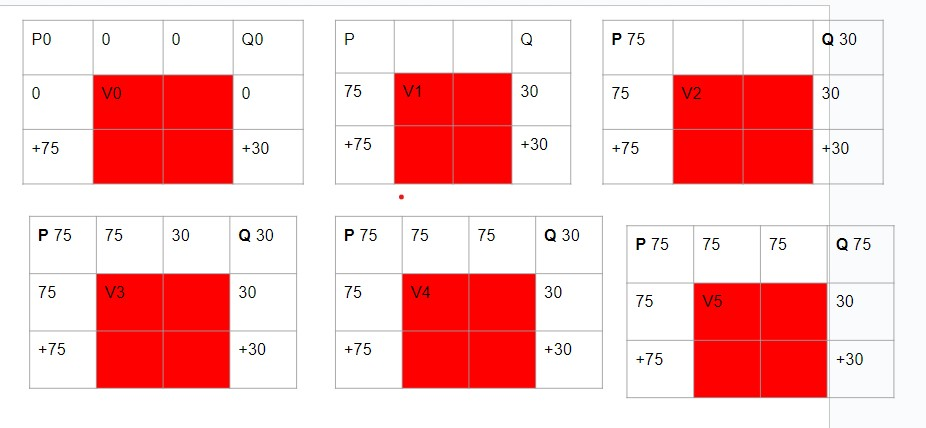
\includegraphics[width=1\textwidth]{q3.jpg}
    \caption{(a) The value iteration process}
    \label{fig:hw6_1}
    \end{figure}

  \item
    \begin{tabular}{llll}
    \hline
    State s & Condition    & i & Vi(s) \\ \hline
    P       & V(P) = V*(P) & 2  & 48     
    \end{tabular}

    %add a image
    \begin{figure}[h]
    \centering
    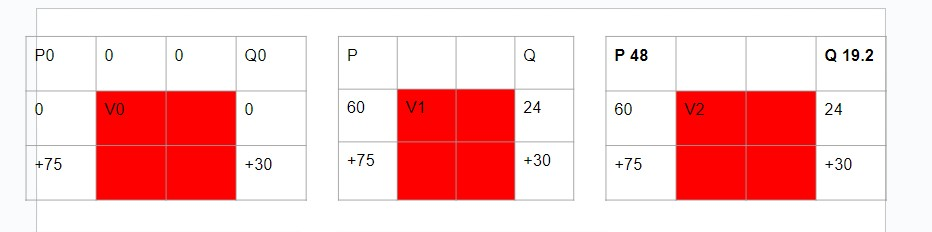
\includegraphics[width=1\textwidth]{q3_2.jpg}
    \caption{(b) The stochastic value iteration process}
    \label{fig:hw6_2}
    \end{figure}
  \end{enumerate}  
\item 
  \begin{enumerate}
    \item  see figures below
      %add image here
      \begin{figure}[h]
      \centering
      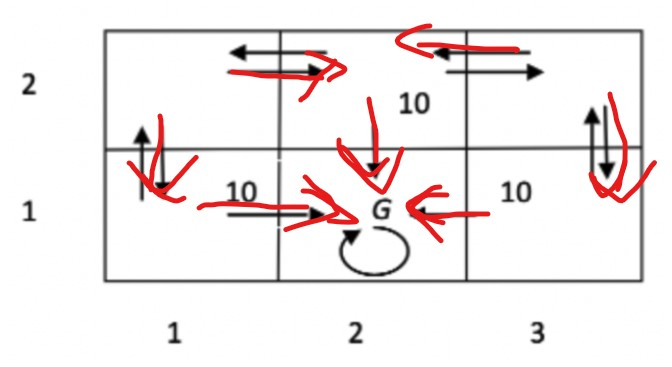
\includegraphics[width=1\textwidth]{q4.jpg}
      \caption{(a) The optimal action}
      \label{fig:hw6_3}
      \end{figure}
    \item V* = 6.4
    \item grid[row2, col1] = 8, grid[row2,col2] = 10, grid[row2, col3] = 8, grid[rpw1, col3] = 10
  \end{enumerate}
\end{enumerate}
\end{document} 